\chapter{Podstawy teoretyczne}


\section{Podstawowe pojęcia}

Niech $\Sigma$ oznacza skończony zbiór o~rozmiarze $|\Sigma| \geq 1$, zwany
dalej alfabetem \cite{taxonomy}. Elementami tego zbioru są symbole (w przypadku tekstu
zwykle utożsamiane z~pojedynczymi literami lub znakami). Alfabet określa się
jako indeksowalny, jeżeli istnieje permutacja indeksów taka, że
$\forall_{i=0..|\Sigma|-1}: a_0 < a_1 < \dots < a_{|\Sigma|-1}$
(symbole mogą być uporządkowane).

Niech $x$ oznacza ciąg symboli (pojęcia symbol, znak i~litera będą
stosowane zamiennie) o~długości $n$.
Element ciągu $x$ występujący na pozycji $i$ oznacza się jako $x[i]$, $i \in
\langle0, n-1\rangle$.
Przez $x[a..b]$, $0 \leq a \leq b \leq n-1$ rozumie się
podciąg $x$ rozpoczynający się na pozycji $a$, a~kończący na pozycji $b$ \cite{gusfield}.
Warto zauważyć, że $x = x[0..n-1]$.

\definicja{Prefiks} to taki podciąg $x$, którego pierwszy element
jest jednocześnie pierwszym elementem ciągu $x$, tj.~$x[0..b]$, $0 \leq b \leq
n-1$.
\definicja{Sufiks} oznacza taki podciąg $x$, którego ostatni element jest
ostatnim znakiem ciągu $x$, tj. $x[a..n-1], 0 \leq a \leq n-1$. Przez
$S^{x}_{i}$ (lub $S_i$ w~przypadku braku niejednoznaczności) rozumie się
sufiks $x[i..n-1]$. Ciąg $x$ jest jednocześnie swoim najdłuższym prefiksem jak i~sufiksem \cite{gusfield}.

\definicja{Konkatenacją} dwóch ciągów $x$ i~$y$ o długości $n$ i~$m$ nazwiemy
ciąg $z$, dla którego $z = x \circ y = x[0] x[1] .. x[n-1] y[0] y[1] .. y[m-1]$.


\section{Struktury danych}

\definicja{Drzewo trie} (\english{trie}) \cite{larsson99structures} jest typem
drzewa przeszukiwań, w~którym węzłom nie odpowiadają klucze, lecz ich fragmenty. W~dalszej
części pracy rozpatrywane będą drzewa, których kluczami są ciągi
symboli z~pewnego alfabetu.\footnote{W nomenklaturze polskiej zarówno
\emph{tree}, jak i~\emph{trie} nazywane są drzewami~\cite{pknuthv3}, str.~528.
O~ile nie będzie powiedziane inaczej, przez drzewo będziemy
rozumieli drzewo \emph{trie}.} W~tego typu drzewach
krawędzie etykietowane są symbolami tego alfabetu, a~,,wartość'' klucza danego węzła wynika z~jego
pozycji i~jest konkatenacją etykiet krawędzi leżących na ścieżce prowadzącej
od korzenia drzewa do tego węzła. Wszystkie podwęzły danego
węzła mają wspólny prefiks równy wartości klucza ich rodzica.
Nieco inny wariant takiego drzewa, nazwany \definicja{drzewem skompresowanym}
(\english{radix tree, Patricia trie}) \cite{larsson99structures}, polega na tym, że węzły
posiadające tylko jednego potomka są z~nimi łączone, a~symbole z~usuniętych
krawędzi są konkatenowane (zob.~rys.~\ref{rys:tree}).

\begin{figure}[t]
    \begin{center}
       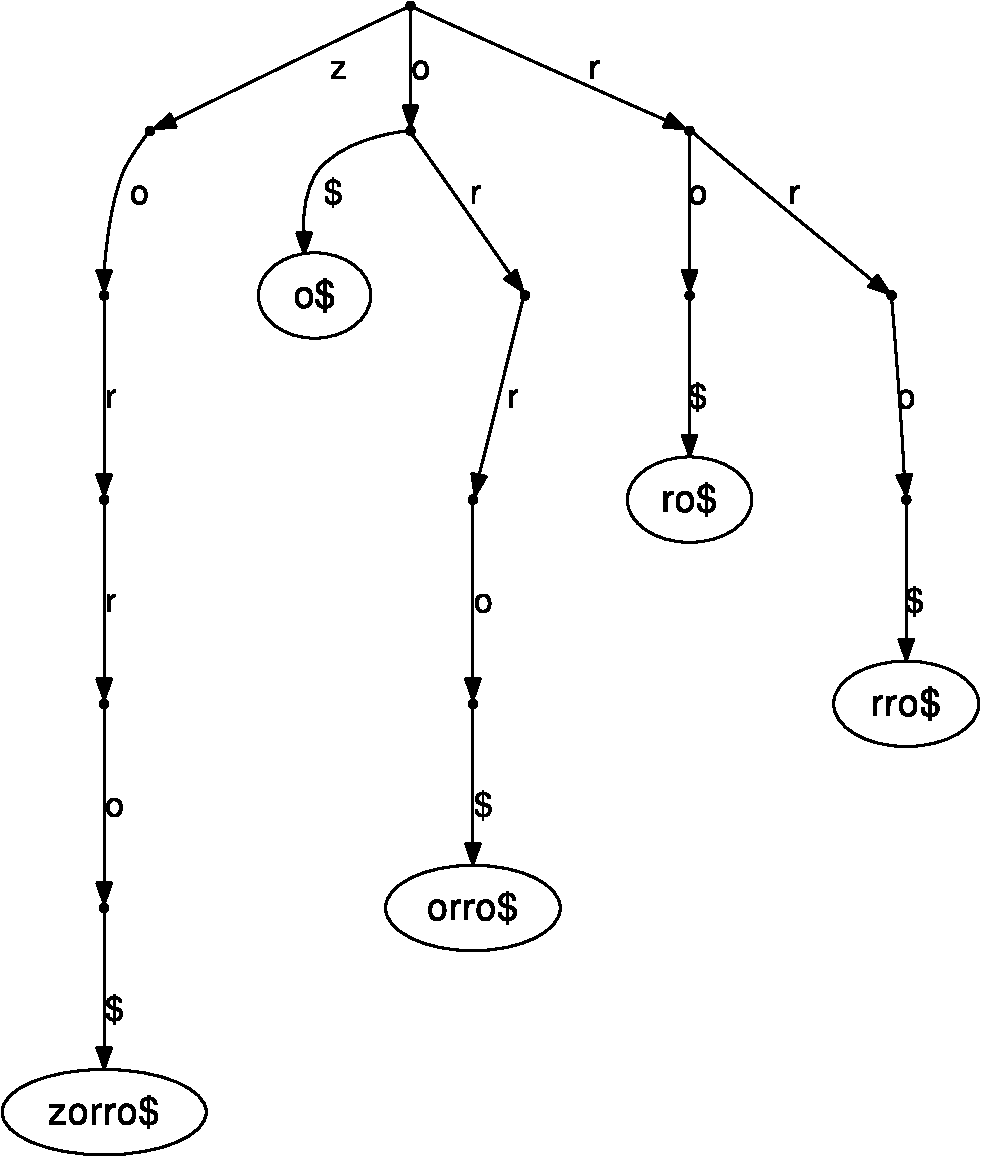
\includegraphics[scale=0.5]{figures/zorroSTrie.pdf}
    \end{center}

    \caption{Drzewo \emph{trie} dla zbioru sufiksów wyrazu ,,zorro'' z~dodanym unikalnym
    symbolem końcowym $\dollar$. Dla
    przejrzystości pominięto łuk od korzenia do liścia o~wartości $\dollar$.}%
    \label{rys:tree}
\end{figure}

\definicja{Drzewo sufiksów} (\english{suffix tree}) \cite{gusfield} dla ciągu symboli
$x$ z~alfabetu $\Sigma$ jest skompresowanym drzewem zbudowanym na zbiorze wszystkich sufiksów
$x$ o~następujących cechach:
\begin{itemize}
  \item krawędzie są etykietowane niepustymi ciągami symboli,
  \item każdy sufiks jest reprezentowany w~drzewie jako ścieżka od korzenia
  do liścia,
  \item wszystkie węzły wewnętrzne drzewa posiadają co najmniej dwóch
  potomków.
\end{itemize}

Zwyczajowo na końcu ciągu $x$ umieszczany jest znak specjalny $\dollar$,
leksykograficznie mniejszy od wszystkich symboli z~alfabetu $\Sigma$. Dzięki temu zabiegowi
żaden sufiks ciągu $x$ nie będzie prefiksem innego sufiksu, co zapewnia zachowanie wszystkich wyżej
wymienionych własności (w przeciwnym przypadku sufiksy mogłyby kończyć się
w~węzłach wewnętrznych drzewa). Rysunek \ref{rys:suffix-tree} prezentuje
drzewo sufiksów dla sekwencji ,,zorro\$''. Trzy ,,klasyczne'' algorytmy
tworzenia drzew sufiksów omówione zostały w~publikacjach \cite{weiner}, \cite{mccreight}
i~\cite{ukkonen}. Ich porównanie można znaleźć w~pracy \cite{from-ukkonen}.

\begin{figure}[t]
    \begin{center}
        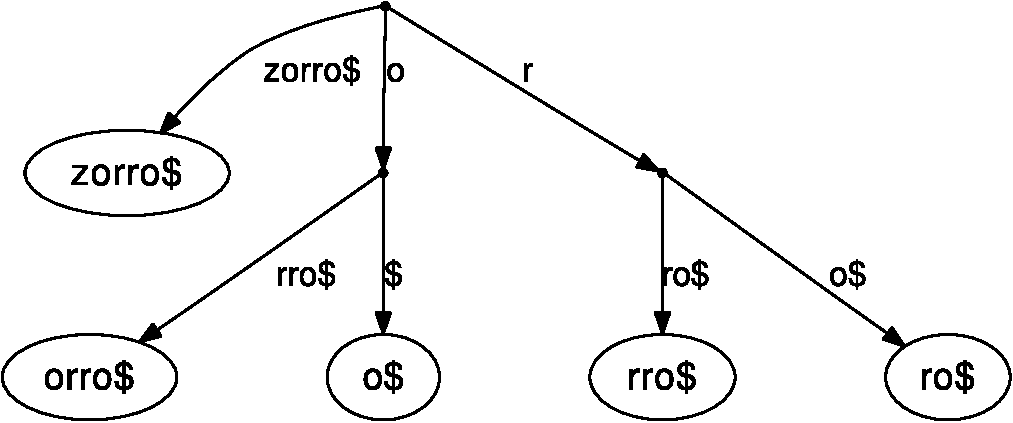
\includegraphics[scale=0.5]{figures/zorroST.pdf}
    \end{center}
    \caption{Drzewo sufiksów wyrazu ,,zorro\$''. Dla przejrzystości pominięto łuk od korzenia do
    liścia o~wartości $\dollar$.}%
    \label{rys:suffix-tree}
\end{figure}

W~literaturze powszechne jest etykietowanie sufiksów pozycją
ich pierwszego symbolu w~słowie $x$ -- przez sufiks o~etykiecie i~rozumie
się podciąg $x[i..n-1]$. \definicja{Tablica sufiksów} (\english{suffix
array}) \cite{taxonomy} słowa $x$~jest tablicą etykiet sufiksów uporządkowaną rosnąco według porządku
leksykograficznego sufiksów.
Tablicę sufiksów słowa $x$ oznacza się $\textit{SA}_x$ lub $\textit{SA}$ jeżeli pominięcie
identyfikatora słowa nie wprowadza niejednoznaczności. Formalnie,
$\textit{SA}[j] = i \iff x[i..n-1]$ jest $j$-tym sufiksem
słowa $x$ według porządku leksykograficznego. Warto zauważyć, że
$\textit{SA}$ jest zawsze permutacją liczb $0..n-1$. Rysunki
\ref{rys:suffix-array-vis} oraz \ref{rys:suffix-array}
prezentują tablicę sufiksów sekwencji symboli ,,zorro\$''.

\begin{figure}[t]
    \begin{center}
        \begin{tabular}{ c c l }
            \toprule
            $j$ & $\textit{SA}[j]=i$ & $x[i..n-1]$ \\
            \midrule
            0 & 5 &        $\dollar$ \\
            1 & 4 &        o$\dollar$ \\
            2 & 1 &        orro$\dollar$ \\
            3 & 3 &        ro$\dollar$ \\
            4 & 2 &        rro$\dollar$ \\
            5 & 0 &        zorro$\dollar$ \\
            \bottomrule
        \end{tabular}
    \end{center}
\caption{Tablica sufiksów dla sufiksów ciągu ,,zorro\dollar''.}%
\label{rys:suffix-array-vis}
\end{figure}

Dla tablicy sufiksów można zbudować \definicja{tablicę najdłuższych wspólnych podciągów}
(\english{longest common prefix array}) \cite{taxonomy} o~długości $n$, której elementy
$\textit{lcp}[i], i = 1..n-1$ oznaczają długość najdłuższego wspólnego prefiksu sufiksów
$\textit{SA}[i]$ i~$\mathit{SA}[i-1]$. Przykładowa tablica najdłuższych wspólnych prefiksów
zaprezentowana jest na rysunku \ref{rys:suffix-array}. Tablicę $\textit{lcp}$ można obliczyć
w~czasie liniowym znając \SA{} zgodnie z~metodami omówionymi w~artykułach \cite{lcp-kasai}
i~\cite{lcp-manzini}.

Strukturą komplementarną do tablicy sufiksów $\textit{SA}$ jest \definicja{odwrotna tablica
sufiksów} (\english{inverse suffix array}) \cite{taxonomy} oznaczana jako $\textit{ISA}$. Jest ona
permutacją liczb $0..n-1$ spełniającą zależność: $\textit{ISA}[i] = j \iff \textit{SA}[j] = i$.
Przykład odwrotnej tablicy sufiksów znajduje się na rysunku \ref{rys:suffix-array}. Wartość $k$-tego
wpisu w~tablicy \SA{} oznacza identyfikator sufiksu na $k$-tej pozycji w~porządku leksykograficznym;
$k$-ty wpis w~tablicy \ISA{} oznacza pozycję sufiksu $k$ w~tablicy \SA{} (oraz w~porządku
leksykograficznym).

\begin{figure}[t]
    \begin{center}
        \begin{tabular}{ r c c c c c c l}
                           & 0 & 1 & 2 & 3 & 4 &  5   &   \\ \cmidrule{2-7}
                   $x = [$ & z & o & r & r & o & $\dollar$ & ] \\
         $\mathit{SA} = [$ & 5 & 4 & 1 & 3 & 2 &  0   & ] \\
        $\mathit{ISA} = [$ & 5 & 2 & 4 & 3 & 1 &  0   & ] \\
        $\mathit{lcp} = [$ & - & 0 & 1 & 0 & 1 &  0   & ] \\
        \end{tabular}
    \end{center}
\caption{Tablica sufiksów $\mathit{SA}$, odwrotna tablica sufiksów $\mathit{ISA}$
oraz tablica najdłuższych prefiksów $\mathit{lcp}$ dla sekwencji
,,zorro\dollar''.}%
\label{rys:suffix-array}
\end{figure}

Przez \definicja{h-grupę} (\english{h-group}) \cite{taxonomy} rozumie się podzbiór
sufiksów słowa $x$ o~wspólnym prefiksie długości $h>0$.
Podział sufiksów na \emph{h-grupy} otrzymuje się poprzez ich częściowe
uporządkowanie ze względu na wartość $h$~pierwszych symboli sufiksu.
Proces ten nosi nazwę \emph{h-sortowania} (\english{h-sort}), w~jego
wyniku sufiksy uporządkowane są według \emph{h-porządku}
(\english{h-order}). Sufiksy należące do jednej \emph{h-grupy} są sobie
równe pod względem \emph{h-porządku}. Algorytmy \emph{h-sortowania}
są zazwyczaj stabilne, czyli zachowują wcześniejszy porządek sufiksów.
Każdej \emph{h-grupie} można przypisać pewien identyfikator
(\english{h-rank}). W~zależności od potrzeb algorytmu, wartości
identyfikatorów dobierane są na jeden z~trzech sposobów:
\begin{enumerate}
  \item grupa identyfikowana jest pozycją pierwszego jej elementu w~przybliżonej tablicy sufiksów -- głowa (\english{head}) grupy,
  \item grupa identyfikowana jest pozycją ostatniego elementu w~przybliżonej
   tablicy sufiksów -- ogon (\english{tail}) grupy,
  \item  każdej z~\emph{h-grup} (nawet jednoelementowym) przypisywane są
  rosnące identyfikatory zgodnie z~kolejnością ich pojawienia się w~$\textit{SA}_h$.
\end{enumerate}

\noindent
Wyniki \emph{h-sortowania} zachowuje się w~\definicja{przybliżonej
tablicy sufiksów} (\english{approximate suffix array}) \cite{taxonomy} oznaczanej
$\textit{SA}_h$. Możliwe jest również wyznaczenie
\definicja{przybliżonej odwrotnej tablicy sufiksów}
(\english{approximate inverse suffix array}) \cite{taxonomy} $\textit{ISA}_h$.
$\textit{SA}_h$ jest permutacją liczb $0..n-1$, natomiast
$\textit{ISA}_h$ może zawierać wartości powtarzające się. Wynika to z~tego,
że każdemu sufiksowi należącemu do danej \emph{h-grupy} przypisywany jest jej identyfikator.
Przykład przybliżonej tablicy sufiksów znajduje się na rysunku \ref{rys:approx-suffix-array}.

\begin{figure}[t]
    \begin{center}
        \begin{tabular}{ r c c c c c c c c c c c c l}
                                 & 0  & 1  & 2  & 3 & 4 & 5   & 6  & 7  & 8 & 9  & 10 & 11     \\ \cmidrule{2-13}
                         $x = [$ & a  & b  & e  & a & c & a   & d  & a  & b & e  & a  &
                       $\dollar$ &]\\ $\mathit{SA}_1 = [$ & 11 & (0 & 3  & 5 & 7 & 10) & (1 & 8) & 4 & 6  & (3 & 9)   & ] \\
            $\mathit{ISA}_1 = [$ & 1  & 6  & 10 & 1 & 8 & 1   & 9  & 1  & 6 & 10 & 1  & 0    & ]\\
                           lub [ & 5  & 7  & 11 & 5 & 8 & 5   & 9  & 5  & 7 & 11 & 5  & 0    & ]\\
                           lub [ & 1  & 3  & 5  & 1 & 3 & 1   & 4  & 1  & 2 & 5  & 1  & 0    & ]\\
        \end{tabular}
    \end{center}
\caption{Przykłady przybliżonej tablicy sufiksów oraz przybliżonej
odwrotnej tablicy sufiksów dla $h=1$. \emph{H-grupy}
wyróżnione zostały nawiasami. Na rysunku przedstawione są 3 wersje tablicy
$\textit{ISA}_1$ różniące się metodami przypisywania identyfikatorów grupom
(wypisane w~kolejności przedstawienia w~tekście).  Źródło: \cite{taxonomy}.}%
\label{rys:approx-suffix-array}
\end{figure}

W~niektórych publikacjach przyjęto inną konwencję nazewniczą, \emph{h-grupa} nazywana
jest tam \emph{h-kubełkiem} lub po prostu \emph{kubełkiem} (\english{bucket}).
Tablica $\textit{ISA}_h$ nazywana jest \definicja{tablicą wskaźników na kubełki}
(\english{bucket pointer array}) \cite{schurmann-phd}.
